\documentclass[../../../main.tex]{subfiles}
\begin{document}

%%%%%%%%%%%%%%%%%%%%%%%%%%%%%%%%%%%%%%%%%
%%%%%%%%%%%%%%%%%%%%%%%%%%%%%%%%%%%%%%%%%
%%%%%%%%%%%%%%%%%%%%%%%%%%%%%%%%%%%%%%%%%
\chapter{How sampling distributions work}

As we saw, sampling distributions end up with a normal shape, where most of the values are clumped together around the population mean, especially if we use a large enough sample size. Why does it work this way? If you think about it, it makes intuitive sense. But it takes a little thinking.


%%%%%%%%%%%%%%%%%%%%%%%%%%%%%%%%%%%%%%%%%
%%%%%%%%%%%%%%%%%%%%%%%%%%%%%%%%%%%%%%%%%
\section{A running example}

Consider a population that has a lot of variance. Suppose, for example, that we want to know the average (mean) height of all high school students in the state Delaware. We cannot measure the height of every high school student in Delaware. That would be too costly and time-consuming. So, we have to take samples. 

We do not know the exact bounds of the population, but let us presume that most Delaware high school students vary quite a lot. We measured a few randomly selected students, and although we don't know the exact bounds, we can tell from our initial measurements that students can be anywhere between 60 inches (5 ft) and 80 inches (about 6 ft, 6 inches). So there's a lot of variation in height among Delaware high school students. 

Also, we do not know the actual average (mean) height of all high school students in Delaware. This actual mean is not known to us. It could be that the mean height is right in the middle, around 70cm. Or it could be that the mean height is lower, around (say) 66cm, or higher, around (say) 74cm. We don't know.


%%%%%%%%%%%%%%%%%%%%%%%%%%%%%%%%%%%%%%%%%
\subsection{Catching all the variations}

Let's think about what happens when we take samples. Taking a sample is like scooping up a random chunk of specimens from the larger collection. And the basic rule is this: the more objects we have in our sample, the more information we have. And the more information we have, the more we know about the population. 

As an analogy, suppose we have a fish tank containing lots of different kinds of fish. Suppose we reach in with a little net that can only scoop up a few fish at once. Are we going to scoop up a representative sample of all the different fish in the tank? No, of course not. We'll only know about a few of the different fish in the tank, because our scoop is only going to catch a couple of them. But now suppose that we reach into the tank with a really big net, that can scoop out a bunch of different fish at once. Are we going to scoop up a representative sample now? Yes, we're much more likely to catch many of the different kinds of fish in our net, because we're scooping up more at once.

The same applies to sampling Delaware high school students. Let's run through some scenarios, to see this.

\begin{enumerate}

  \item \textbf{Small samples}. Suppose we take a small sample. For instance, suppose we randomly select only 3 students. We measure their heights, and then we calculate the average (mean) height of those 3 students. Because we've only selected 3 students, we cannot get much information about the population.
  
  \begin{enumerate}
  
    \item We might (just by chance) select 3 very short students (say, all around 60 inches). The mean of this sample will be low, around 60 inches. It is very unlikely that this sample represents the whole population (unless most Delaware high school students are also very short, around 60 inches). This sample is bad, because we've missed students with different heights. We haven't included any tall students, for example.
    
    \item We might (by chance) select 3 very tall students (say, all around 80 inches). The mean of this sample will be high, around 80 inches. But it is very unlikely that this sample represents the whole population, unless most students happen to be very tall. This sample is bad, because we've missed students with different heights (for instance, shorter heights).
    
    \item We might (by chance) get one student near 60 inches, one near 80 inches, and one in the middle, near 70 inches. The mean of this sample will be near the middle. Would this represent the whole population well? Only if the whole population happens to have an average in the middle, which may or may not be the case. What if the actual average is, say, 66 inches, or 74 inches? Then our sample is not accurate. This sample is bad too, because it doesn't have enough specimens to push the average towards the correct number.
    
    \item We might (by chance) get a clump of students whose mean falls near some other value, like 76 inches. Does this represent the larger population? Again, only if the larger population happens to have an average near 76 inches, and that seems unlikely. This sample is bad too, because it's missing too many other representative heights. There are too many other students, with different heights, that are missing from this sample.
  
  \end{enumerate}
  
  Selecting only 3 students gives us so little information, that we simply cannot tell much about the larger population. By selecting 3, we only scooped up a few students. There are just too many other students with different heights missing from our sample. 
  
  \item \textbf{Larger samples}. Suppose that we take a much larger sample. Suppose we randomly select 100 students, and calculate the mean of their heights.
  
  \begin{enumerate}

    \item It is of course possible that (just by chance) we happen to get 100 really tall students. If this were to happen, then the mean of the sample would be high, and it would not represent the population very well. It would be skewed towards tall students. But since we've selected such a large number of students, it seems quite unlikely that we would happen to get \emph{all} tall students. 
    
    \item It is of course possible (just by chance) that we happen to get 100 very short students, so that our sample mean turns out to be very low. But again, since we've selected so many students, this seems very unlikely.
    
    \item What seems much more likely is that some of the students in our sample will be tall, some will be short, some will be in the middle, and so on. In fact, it seems that we will very likely get a sample of students that represent the population well. If the population has students with uniformly distributed heights, then our sample will probably have uniformly distributed heights. If the population has a bulge of heights around (say) 74 inches, then our sample will probably have a bulge of heights around (say) 74 inches too. 

  \end{enumerate} 
  
  Selecting a much larger sample gives us more information about the population. Because we select more students (we select 100 instead of just 3), we have a much greater chance of catching most of the different variations in our sample.

  \item \textbf{Very large samples}. Suppose that we select a very large number of students for our sample. For example, suppose we select 1000 students, we measure their heights, and compute a mean for them. Is this sample going to represent the larger population? 
  
  \begin{enumerate}
  
    \item It is still possible that we might just happen to select (say) 1000 tall students, and entirely by chance we miss most of the other variations in the larger population. But this seems \emph{extremely} unlikely now, because we've taken such a large sample.
    
    \item Our scoop is so big that it seems much more likely that we will end up catching most of the variations of heights.
  
  \end{enumerate}
  
  So a much larger scoop is going to give us more information, because we're going to catch more of the variations.

\end{enumerate}


%%%%%%%%%%%%%%%%%%%%%%%%%%%%%%%%%%%%%%%%%
\subsection{The effect on the plot}

So we know that larger sample sizes are going to catch more of the variations, and so the sample mean is going to be closer to the actual population mean. 

Think about our example above. With only 3 students in our scoop, the mean of the sample could be wildly far off from the mean of the population. What do we call it when the value is far away from the mean? That's the \vocab{variance}, and from the variance we also have the \vocab{standard deviation}. 

What does a high variance/STDEV do to a normal curve? It makes it wider and flatter. For example, here is a normal curve:

\begin{center}
  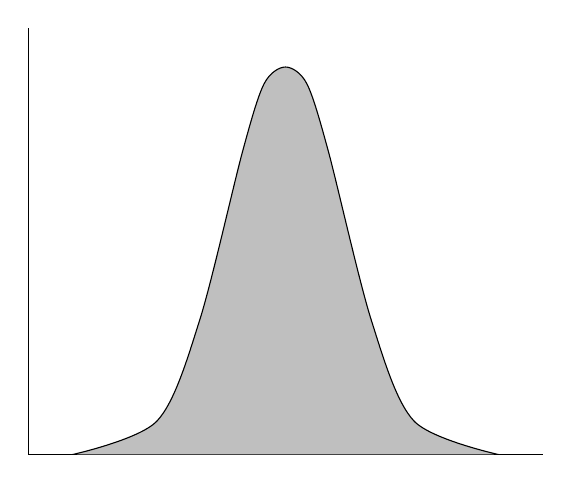
\begin{tikzpicture}
    \begin{axis}[
      axis lines*=left,
      ytick=\empty,
      xtick=\empty,
      height=7cm,
      enlarge y limits={value=0.1,upper},
      ]
      \addplot[smooth, fill=lightgray, domain=0:10] 
        coordinates{
          (0, 0) (2, 0.5) (3, 2) (4, 4.5) (4.5, 5.5)
          (5, 5.75)
          (5.5, 5.5) (6, 4.5) (7, 2) (8, 0.5) (10, 0)} 
        \closedcycle;

    \end{axis}
  \end{tikzpicture}
\end{center}

\noindent
If we mark the standard deviations, we can see how the curve gets pushed out from the middle (the mean $\populationmean$), depending on how far away from the middle each deviation is:

\begin{center}
  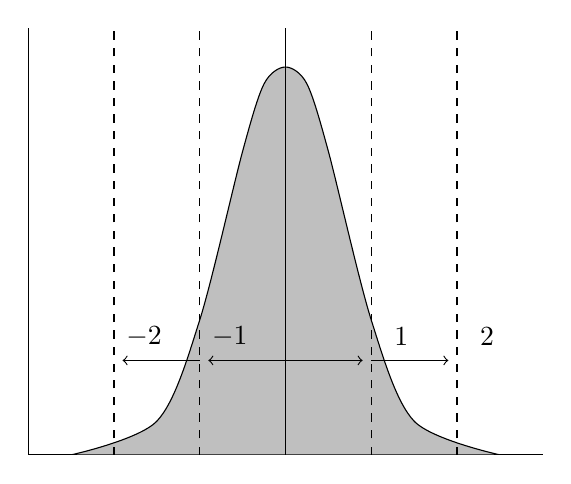
\begin{tikzpicture}
    \begin{axis}[
      axis lines*=left,
      ytick=\empty,
      xtick=\empty,
      height=7cm,
      enlarge y limits={value=0.1,upper},
      ]
      \addplot[smooth, fill=lightgray, domain=0:10] 
        coordinates{
          (0, 0) (2, 0.5) (3, 2) (4, 4.5) (4.5, 5.5)
          (5, 5.75)
          (5.5, 5.5) (6, 4.5) (7, 2) (8, 0.5) (10, 0)} 
        \closedcycle;
        
      \draw (5, 0) -- (5, 10);
      \node at (5.5, 1.75) {$\populationmean$};
      
      \draw[dashed] (7, 0) -- (7, 10);
      \node at (7.7, 1.75) {$1\populationstdev$};
      \draw[->] (5, 1.4) -- (6.8, 1.4);
      \draw[dashed] (9, 0) -- (9, 10);
      \node at (9.7, 1.75) {$2\populationstdev$};
      \draw[->] (7, 1.4) -- (8.8, 1.4);
      
      \draw[dashed] (3, 0) -- (3, 10);
      \node at (3.7, 1.75) {$-1\populationstdev$};
      \draw[->] (5, 1.4) -- (3.2, 1.4);
      \draw[dashed] (1, 0) -- (1, 10);
      \node at (1.7, 1.75) {$-2\populationstdev$};
      \draw[->] (3, 1.4) -- (1.2, 1.4);
    \end{axis}
  \end{tikzpicture}
\end{center}

\noindent
If there is a larger deviation, the curve gets pushed out even more (it gets wider and flatter):


\begin{center}
  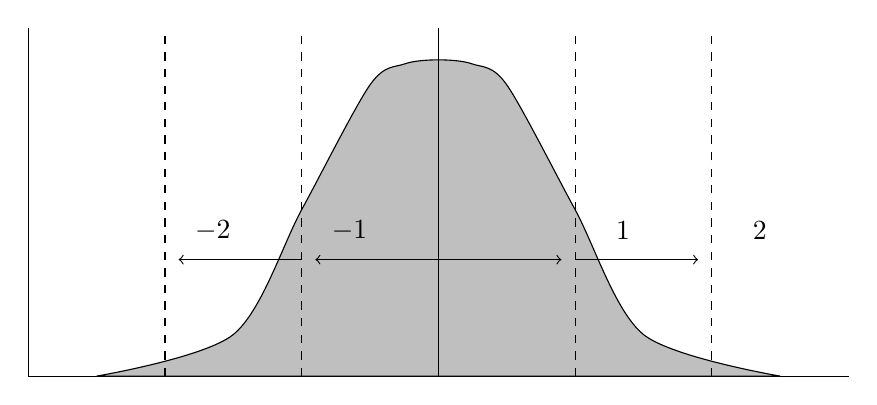
\begin{tikzpicture}
    \begin{axis}[
      axis lines*=left,
      ytick=\empty,
      xtick=\empty,
      height=6cm,
      width=12cm,
      enlarge y limits={value=0.1,upper},
      ]
      \addplot[smooth, fill=lightgray, domain=0:10] 
        coordinates{
          (0, 0) (2, 0.5) (3, 2) (4, 3.5) (4.5, 3.75)
          (5, 3.8)
          (5.5, 3.75) (6, 3.5) (7, 2) (8, 0.5) (10, 0)} 
        \closedcycle;
        
      \draw (5, 0) -- (5, 10);
      \node at (5.5, 1.75) {$\populationmean$};
      
      \draw[dashed] (7, 0) -- (7, 10);
      \node at (7.7, 1.75) {$1\populationstdev$};
      \draw[->] (5, 1.4) -- (6.8, 1.4);
      \draw[dashed] (9, 0) -- (9, 10);
      \node at (9.7, 1.75) {$2\populationstdev$};
      \draw[->] (7, 1.4) -- (8.8, 1.4);
      
      \draw[dashed] (3, 0) -- (3, 10);
      \node at (3.7, 1.75) {$-1\populationstdev$};
      \draw[->] (5, 1.4) -- (3.2, 1.4);
      \draw[dashed] (1, 0) -- (1, 10);
      \node at (1.7, 1.75) {$-2\populationstdev$};
      \draw[->] (3, 1.4) -- (1.2, 1.4);
    \end{axis}
  \end{tikzpicture}
\end{center}

\noindent
The same thing happens with sampling distributions. If you have a lot of variance in your sample, then the curve is going to be wider and flatter. If you have much less variance, then the curve is going to be taller and skinnier. 

\begin{itemize}

  \item For instance, if you have a bunch of samples of 3 students only, you will have a lot of variation from sample mean to sample mean. One mean might be near 60 inches, and another might be near 70 inches. So you'll have lots of means that are very different from each other. Consequently, the plot of all those 3-student sample means will be wide and flat, because the variance/STDEV is quite big.
  
  \item By contrast, if you have a bunch of samples of 100 students, you will have much tighter curve. This is because the means you get from sample to sample will be much closer to each other. With 100 students in each sample, the means will not be so wildly different from each other. They will all be much closer. Hence, the variance/STDEV of all those means will be smaller, and the plot of all those sample means will be taller and skinnier. 
  
\end{itemize}

\noindent
This should make good sense. We take a sample because we want a representative of the larger population. When we take a sample and calculate the mean of that sample, we're trying to approximate or estimate the mean of the larger population. 

So, how good our estimates are should be reflected in how tightly our sample means bunch around the center (the mean) of the plot.

\begin{itemize}

  \item If we use small samples, like 3 students, we don't get very good estimations of the larger population mean. Our samples are all over the place. Hence, the plot will be a lot wider, which indicates that we're getting sample means that can be quite a long way away from the mean.
  
  \item If we take larger samples, like 100 students, we get much better estimations of the larger population mean. Our sample means should all sit a lot closer to the mean.

\end{itemize}

\noindent
Earlier, I pointed out that the mean of a sampling distribution gets closer and closer to the mean of the population, if our samples are large enough. This should make sense now. 

\begin{itemize}

  \item If we build a sampling distribution with samples that are very small, we end up getting a lot of sample means that are all over the place. Hence, we get a very wide plot. The plot shows us (visually) that our sample means are not bunched very tightly around the actual mean of the population. And that makes sense, because with small samples, our sample means can be quite a long way from the real population mean.

  \item If we build a sampling distribution with samples that are big, we end up getting a lot of sample means that are close to the mean of the plot. The plot shows us that our sample means are bunched much more tightly near the actual mean of the population. And that makes senes, because with larger samples, our means should in fact be closer to the real population mean.

\end{itemize}


%%%%%%%%%%%%%%%%%%%%%%%%%%%%%%%%%%%%%%%%%
\subsection{The standard error}

Remember what we just said: a larger sample has a tighter plot, and smaller sample has a wider plot. So, we would expect that the width/spread of a sampling distribution should be related to the size of the sample, and of course the variance/STDEV of the raw population data itself.

It turns out that this is indeed the case. It turns out that the standard deviation of the \emph{sampling distribution} is always the same as the standard deviation of the \emph{larger population}, divided by the square root of the \emph{sample size}:

\begin{equation*}
  \frac{\populationstdev}{\sqrt{\samplesize/}}
\end{equation*}

\noindent
In a sampling distribution, we call the standard deviation the \vocab{standard error}. This is just another name for the same thing: the \emph{standard error} is just the standard deviation of a \emph{sampling distribution}. We can write ``standard error'' as ``$\StdErr/$'' for short, so the equation is:

\begin{equation*}
  \StdErr/ = \frac{\populationstdev}{\sqrt{\samplesize/}}
\end{equation*}

\noindent
Think about what this formula says. It says that first we take the standard deviation of the larger population, $\populationstdev$, whatever it may be. Naturally, the larger population has its own variance/STDEV. The values are spread out from the mean to some extent, and that amount is the variance/STDEV. So, we need to start with whatever variance there is in the original population data.

But then, we take the sample size (i.e., how many specimens we take in our sample), and we divide $\populationstdev$ by the square root of that. So, think about what that does:

\begin{itemize}
  \item If the sample size is bigger, we will end up dividing $\populationstdev$ by a bigger number.
  \item If the sample size is smaller, we will end up dividing $\populationstdev$ by a smaller number.
\end{itemize}

\noindent
And what does dividing by a bigger or smaller number do? 

\begin{enumerate}
  \item As you divide a number $x$ by a bigger and bigger number, the result gets smaller and smaller. 
  \item As you divide a number $x$ by a smaller and smaller number, the result gets bigger and bigger.
\end{enumerate}

\noindent
For example:

\begin{equation*}
  \frac{10}{1} = 10 \hskip 0.5cm \frac{10}{5} = 2 \hskip 0.5cm \frac{10}{10} = 1 \hskip 0.5cm \frac{10}{1000} = 0.01
\end{equation*}

\noindent
This applies to the $\StdErr/$ of a sampling distribution too:

\begin{itemize}

  \item As the sample size gets bigger, we divide $\populationstdev$ by a bigger number, which makes the result smaller. So the $\StdErr/$ (the standard deviation) of the sampling distribution gets smaller as the sample size gets bigger. Hence, the plot will get skinnier and skinnier for bigger samples.
  
  \item Conversely, as the sample size gets smaller, we divide $\populationstdev$ by a smaller number, which makes the result bigger. So the $\StdErr/$ (the standard deviation) of the sampling distribution gets bigger as the sample size gets smaller. Hence, the plot gets fatter and fatter for smaller samples.

\end{itemize}


%%%%%%%%%%%%%%%%%%%%%%%%%%%%%%%%%%%%%%%%%
\subsection{Summary}

Intuitively, this all makes sense. Remember this:

\begin{quote}
  A sampling distribution of sample means approximates the actual mean of the population that the samples are taken from.
\end{quote}

\noindent
Consequently, the sampling distribution should look like a normal curve, where the sample means cluster around the real mean of the larger population. 

The spread of the sampling distribution should be affected though, by the size of the samples:

\begin{itemize}
  \item As samples get bigger, the sample means get closer to the real mean. So we should expect the sampling distribution to have its values cluster more tightly around the middle point for bigger sample sizes. Hence the normal curve should be skinnier for bigger samples.
  \item Conversely, for smaller sample sizes, we should expect the values to be spread farther and farther away from the middle point. Hence the normal curve should be fatter for smaller samples.
\end{itemize}



%%%%%%%%%%%%%%%%%%%%%%%%%%%%%%%%%%%%%%%%%
%%%%%%%%%%%%%%%%%%%%%%%%%%%%%%%%%%%%%%%%%
\section{Notation}

We refer to a random variable with a big ``X,'' like this:

\begin{equation*}
  \RandVar/
\end{equation*}

\noindent
Talking about sample means is so common though, that we use a special symbol for it. We symbolize the sample means like this:

\begin{equation*}
  \SamplingRandVar/
\end{equation*}

\noindent
We call this ``$X$-bar'' (or even ``big $X$-bar''). 

It is a random variable, just like any other random variable. We can describe it with words:

\begin{equation*}
  \SamplingRandVar/ = \text{ the mean of a sample }
\end{equation*}

\noindent
When we want to refer to the possible values that a random variable $\RandVar/$ can take on, we write a little ``x,'' like this:

\begin{equation*}
  \RandVarVal/
\end{equation*}

\noindent
For example, we might talk about when $\RandVar/$ has a value of 5, by writing this:

\begin{equation*}
  \RandVarVal/ = 5
\end{equation*}

\noindent
When we want to talk about the values that a sampling random variable $\SamplingRandVar/$ can take on, we write a little ``x''' as well, but we put a bar over it:

\begin{equation*}
  \SamplingRandVarVal/
\end{equation*}

\noindent
We call this ``$x$-bar'' (or even ``little $x$-bar'').

So, for example, if we want to talk about when $\SamplingRandVar/$ has a value of 5.203, we can write this:

\begin{equation*}
  \SamplingRandVarVal/ = 5.203
\end{equation*}

\noindent
When we want to refer to the mean of a population, we normally write this:

\begin{equation*}
  \populationmean
\end{equation*}

\noindent
When we want to refer to the mean of a sample means distribution, we add a subscripted little $x$-bar:

\begin{equation*}
  \SamplingMean/
\end{equation*}

\noindent
When we want to refer to the standard deviation of a sampling distribution (which is called the ``standard error''), we write this:

\begin{equation*}
  \frac{\populationstdev}{\sqrt{\samplesize/}}
\end{equation*}

\noindent
Or, sometimes, we just write this:

\begin{equation*}
  \StdErr/
\end{equation*}

%%%%%%%%%%%%%%%%%%%%%%%%%%%%%%%%%%%%%%%%%
%%%%%%%%%%%%%%%%%%%%%%%%%%%%%%%%%%%%%%%%%
\section{The Central Limit Theorem}

I've pointed out already that sampling distributions always tend to approach a normal distribution, and the mean of a sampling distribution (which we symbolize as $\SamplingMean/$) always tends to approach the mean of the population (symbolized as $\populationmean$) which the samples are taken from.

To be more exact, we should say that, if the sample size $\samplesize/$ is big enough, then the sampling distribution will approach the normal distribution, and its mean will approach the population's mean.

Think of this as a law of statistics, analogous to (say) the laws of physics. It always holds true. It has a name too. We call it the \vocab{Central Limit Theorem}, or \CLT/ for short. 

There are many ways to describe the \CLT/. For our purposes here, if we need to state the \CLT/ in words, we can just say something like this:

\begin{quote}
  The Central Limit Theorem states that, if the sample size is large enough, then a sampling distribution constructed from those samples will approximate a normal distribution.
\end{quote}

\noindent
Mathematically, there are different ways to state the \CLT/ too. For our purposes here, we will simply assume that we are talking about sample means, and we can say that the distribution of sample means will always have a normal distribution with a mean $\SamplingMean/$ and a standard error $\frac{\populationstdev}{\sqrt{\samplesize/}}$. So if we need to write down the \CLT/ using mathematical symbols, we can just write this:

\begin{equation*}
  \SamplingRandVar/ \sim N(\SamplingMean/, \frac{\populationstdev}{\sqrt{\samplesize/}})
\end{equation*}


%%%%%%%%%%%%%%%%%%%%%%%%%%%%%%%%%%%%%%%%%
\subsection{Some details}

Here are some details to remember:

\begin{enumerate}

  \item The \CLT/ works for any statistic that we can compute for a sample. It works for means, proportions, sums, or what-have-you. But we will most commonly speak about sample means, so we will tend to speak about the \CLT/ as if it only applies to sample means. 

  \item A sampling distribution is built by taking sample after sample from a population, computing a statistic (like the mean) for each sample, and then adding each statistic to a collection.
  
    \item Sampling is done with replacement. So, you take your samples, and then put them back. In subsequent samples, you very well might get some of the same specimens again.
  
  \item Since sampling is done with replacement, there is no limit to how many samples can be taken. We can sample and sample forever.
  
  \item In fact, a sampling distribution is a kind of theoretical entity. Obviously it is impossible to keep sampling forever. But when we think about sampling distributions, we assume or imagine that they are completed, being built from the \emph{infinite} number of samples that can be taken from the target population.

  \item For large enough sample sizes, a sampling distribution will always approximate a normal distribution. What this means is that, as we add more and more samples to the distribution, the shape gets closer and closer to a normal curve.
  
  \item For large enough sample sizes, the mean of a sampling distribution $\SamplingMean/$ will approximate the mean $\populationmean$ of the population the samples are taken from. What this means is that, as we add more and more samples to the distribution, $\SamplingMean/$ will get closer and closer to $\populationmean$.

  \item A sampling distribution is constructed from samples that are all the same size. That is, the size for a sampling distribution is fixed. We refer to the size as $\samplesize/$. So you can't build a sampling distribution from some samples that have 10 specimens ($\samplesize/ = 10$), and others that have 15 specimens ($\samplesize/ = 15$). Every sample in a sampling distribution must have exactly the same size (e.g., they must all have 10 specimens, or they must all have 15 specimens, or whatever). 
  
  \item The \CLT/ works best for larger sample sizes. How big does a sample need to be? It depends, but a rough guide is: 30. 
  
  \item The shape of the population doesn't matter. Any sampling distribution built from samples taken from a population will always be normal (if the sample size is big enough). Even if the population has a crazy, totally irregular shape, the sampling distribution will turn out to be normal!
  
  \item If the population is already normal, then the sample size can be smaller. For normally distributed populations, sampling distributions will approach a normal curve with even smaller sample sizes.
  

\end{enumerate}


%%%%%%%%%%%%%%%%%%%%%%%%%%%%%%%%%%%%%%%%%
\subsection{A theorem?}

The \CLT/ is a theorem of statistics. What is a theorem? A theorem is any mathematical statement, which has been rigorously proven to be correct. 

A mathematical proof of a theorem shows that it is impossible for the theorem to be false. Such a proof will examine every possible way that things can turn out, and show that no matter what, the statement will always be true.

The \CLT/ is a theorem in just this sense. There are actually a number of different proofs, but they all show that no matter what your population data is shaped like, a sampling distribution built from large enough samples will always turn out to be normal.


\end{document}
